% !TeX root = ../main.tex
\section{Introduction}
Mixture-of-experts (MoE) models increase capacity by adding experts while activating only a few of them for each token~\cite{shazeer,switch,mixtral,deepseekmoe}.
Sparse activation limits computation while inference still needs access to the full expert pool.
On a single GPU, high-bandwidth memory (HBM) holds only part of that pool.
Host memory provides more space.
Dense weights, activations, and the KV cache also use it.
When expert weights exceed the combined space available in HBM and host memory, the remaining weights reside on a hard disk drive (HDD).
An HBM hit executes without moving expert weights; a host hit needs a host-to-device transfer; a miss in both tiers needs an HDD read as well.
The router makes these choices relevant at every MoE layer and for every token.
An HDD read during prompt processing delays the first token, and a read during generation delays a later token.
We study how to place and retain experts across these tiers while keeping the original weights and routing decisions.

Prior systems use CPU--GPU offloading to serve experts beyond GPU capacity~\cite{offloading,fiddler,lightning}.
Expert caches keep selected weights in memory~\cite{swapmoe,moeinfinity}, and storage-aware systems address reads from slower devices~\cite{flashmoe}.
MoE-CORE allocates GPU slots across layers~\cite{core}, while SSD-LLaMA updates RAM/VRAM caches from access history~\cite{ssdllama}.
Demand also differs across layers, making the choice of initial residents part of the problem.
Independent HBM and CPU admission can spend two cache slots on the same expert while another requested expert remains on HDD.
Figure~\ref{fig:intro}(a) follows an on-demand path.
The first request reads an expert from HDD, and a later request reads it again after both memory tiers evict it.
The figure also shows a task change: new requests select different experts while memory still holds weights from the earlier task.
Initial placement affects the first read; retention determines whether the later read is needed; updating cache membership determines which task uses the available slots.
Our approach allocates both HBM and CPU slots across layers before serving and links HBM replacement to CPU admission during serving.

\begin{figure}[!t]
\centering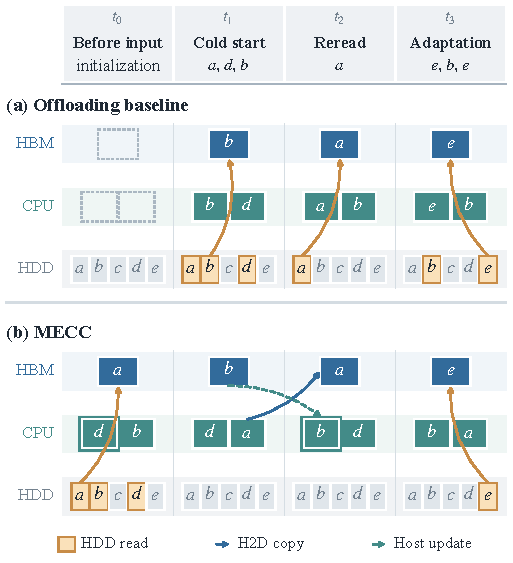
\includegraphics[width=\columnwidth]{figures/fig01_demand_lifecycle.pdf}
\par\nointerlineskip
\caption{Offloading baseline (a) and MECC (b), each with one HBM and two CPU slots. Orange paths mark HDD reads; dashed links mark host updates.}
\label{fig:intro}
\end{figure}

We present \mecc{} (MoE Expert Cache Coordination) to manage initial placement and serving-time updates through the same per-layer HBM/CPU cache state.
Before deployment, MECC analyzes recorded expert selections, allocates slots across layers, and selects their initial expert residents.
It budgets host memory for resident copies and transfer buffers.
During inference, each routed access uses that state to select a source tier for delivery and to update a joint HBM/CPU recency order.
The updated resident sets become the state seen by the next access.
An HBM hit changes recency without moving weights; a CPU hit or an HDD miss can also change which experts occupy the two tiers.
Figure~\ref{fig:intro}(b) shows how the two tiers update together: promoting a CPU resident to HBM releases its host slot and displaces an HBM resident.
MECC assigns the displaced expert's existing host copy to the released slot, keeping it available for a later request without a device-to-host transfer.
An expert absent from both resident tiers comes from HDD; during prefill, its read can overlap GPU work on another expert.
Delivery completes the required transfer before expert execution.
The planner's per-layer capacities bound each update.
The state carries across token and request boundaries, so a later task starts from the residents left by earlier accesses.
It can admit newly requested experts under the same capacities without rerunning placement.

Our contributions are as follows.
\begin{list}{}{\setlength{\leftmargin}{16pt}\setlength{\labelwidth}{14pt}\setlength{\labelsep}{2pt}\setlength{\itemsep}{3pt}\setlength{\topsep}{3pt}}
\item[(1)] We propose an expert planner for MoE deployment on one GPU.
It allocates HBM/CPU capacity across layers by marginal demand coverage and selects initial expert residents using offline routing analysis.
\item[(2)] We propose a retention mechanism that reuses CPU slots released by promotion.
It links HBM replacement to CPU admission, keeping the displaced expert's host copy available for reuse and saving a device-to-host transfer.
\item[(3)] We propose a request-driven policy that adapts expert residency to changes in task demand.
The policy updates the initial resident set through a joint HBM/CPU recency order, preserving per-layer capacities and cache state across tokens and requests.
\end{list}
We evaluate TPOT and TTFT on three models across A100 and H100 GPUs.
MECC reaches up to 1.25$\times$ speedup in TPOT and 1.19$\times$ in TTFT on A100.
The implementation is available at \url{https://anonymous.4open.science/r/MECC-949C/}.
